\documentclass[11pt,a4paper]{article}
\usepackage[T1]{fontenc}
\usepackage[utf8]{inputenc}
\usepackage{lmodern}
\usepackage{amsmath,amssymb,amsthm,mathtools,mathrsfs}
\usepackage{graphicx,float,xcolor,multicol}
\usepackage[shortlabels]{enumitem}
\usepackage[margin=27mm]{geometry}
\usepackage{microtype,needspace,placeins}
\usepackage{tikz,tikz-cd}
\usetikzlibrary{arrows.meta,calc,positioning,patterns,decorations.pathreplacing}
\usepackage[colorlinks=true,linkcolor=teal,urlcolor=teal,citecolor=teal]{hyperref}
\setlength{\parindent}{0pt}
\setlength{\parskip}{.6em}
\setcounter{secnumdepth}{0}
\allowdisplaybreaks
\raggedbottom
\providecommand{\cross}{\times}
\DeclareUnicodeCharacter{2020}{\ensuremath{\dagger}}
\DeclareMathOperator{\supp}{supp}
\DeclareMathOperator*{\esssup}{ess\,sup}
\providecommand{\chapter}{\section}
\newenvironment{tool}[2]{\subsection*{Tool #1 --- #2}}{}
\newcommand{\ToolRef}[1]{Tool #1}
\newcommand{\FigureTag}[2]{\textit{Figure #1}}
\newcommand{\Result}[1]{\subsection*{#1}}
\newcommand{\Application}[1]{\subsubsection*{Application\if\relax\detokenize{#1}\relax\else\space--- #1\fi}}
\newcommand{\ProofHeading}{\par\textit{Proof.}\space}
\newcommand{\ProofOf}[1]{\par\textit{Proof of #1.}\space}
\newcommand{\RemarkHeading}{\par\textbf{Remark.}\space}
\newcommand{\NoteHeading}{\par\textbf{Note.}\space}
\newcommand{\ExerciseHeading}{\par\textbf{Exercise.}\space}

% Rendering support only; mathematical text is in each independent post.
\usepackage{booktabs,array,longtable}
\definecolor{HandoutBlue}{HTML}{2F6690}
\definecolor{HandoutNavy}{HTML}{17365D}
\newtheorem{theorem}{Theorem}
\newtheorem{lemma}[theorem]{Lemma}
\newtheorem{proposition}[theorem]{Proposition}
\newtheorem{corollary}[theorem]{Corollary}
\newtheorem{conjecture}[theorem]{Conjecture}
\newtheorem{definition}{Definition}
\newtheorem{example}{Example}
\newtheorem{namedtoolcounter}{Tool}
\newenvironment{namedtool}[1]{\begin{namedtoolcounter}[#1]}{\end{namedtoolcounter}}
\newtheorem*{claim}{Claim}
\newtheorem*{remark}{Remark}
\newtheorem*{exercise}{Exercise}
\newtheorem*{question}{Question}
\newtheorem*{observation}{Observation}
\newcommand{\SourceChapter}[2]{\section*{#2}}
\newcommand{\Lecture}[2]{\section*{Lecture #1: #2}}
\newcommand{\unclear}[1]{\textit{[unclear: #1]}}
\newcommand{\sourcegap}{\textit{[unfinished in the source]}}
\DeclareMathOperator{\dist}{dist}
\DeclareMathOperator{\id}{id}
\DeclareMathOperator{\Hol}{Hol}
\DeclareMathOperator{\Per}{Per}
\DeclareMathOperator{\Fix}{Fix}
\DeclareMathOperator{\diam}{diam}
\DeclareMathOperator{\Var}{Var}
\DeclareMathOperator{\Leb}{Leb}
\DeclareMathOperator{\Hom}{Hom}
\DeclareMathOperator{\End}{End}
\DeclareMathOperator{\Ann}{Ann}
\DeclareMathOperator{\Spec}{Spec}
\DeclareMathOperator{\Max}{Max}
\DeclareMathOperator{\Ob}{Ob}
\DeclareMathOperator{\Tor}{Tor}
\DeclareMathOperator{\Ass}{Ass}
\DeclareMathOperator{\Mor}{Mor}
\DeclareMathOperator{\Fun}{Fun}
\DeclareMathOperator{\Nat}{Nat}
\DeclareMathOperator{\Cone}{Cone}
\DeclareMathOperator{\MCG}{MCG}
\DeclareMathOperator{\Aut}{Aut}
\DeclareMathOperator{\Deck}{Deck}
\DeclareMathOperator{\SL}{SL}
\DeclareMathOperator{\PSL}{PSL}
\DeclareMathOperator{\Area}{Area}
\DeclareMathOperator{\im}{im}
\DeclareMathOperator{\PSh}{PSh}
\newcommand{\CRing}{\mathsf{CRings}}
\newcommand{\AMod}{A\text{-}\mathsf{Mod}}
\newcommand{\Ab}{\mathsf{Ab}}
\newcommand{\Z}{\mathbb Z}
\newcommand{\Q}{\mathbb Q}
\newcommand{\R}{\mathbb R}
\newcommand{\C}{\mathbb C}
\newcommand{\N}{\mathbb N}
\newcommand{\kk}{\mathbb k}
\renewcommand{\aa}{\mathfrak a}
\newcommand{\bb}{\mathfrak b}
\newcommand{\pp}{\mathfrak p}
\newcommand{\qq}{\mathfrak q}
\newcommand{\mm}{\mathfrak m}
\newcommand{\nn}{\mathfrak n}
\newcommand{\rad}{\mathrm r}
\newcommand{\cat}[1]{\mathsf{#1}}
\setcounter{secnumdepth}{0}
\allowdisplaybreaks

\graphicspath{{figures/complex-dynamics-notes/}}
\begin{document}
\section*{Quasiconformal Mappings}
% BLOG-CONTENT-BEGIN
The dynamics of a map \(f:S\to S\) is a topological invariant. Fixed points, critical points, and the nature of periodic orbits---attracting, repelling, superattracting, parabolic, or non-linearizable---remain as they were when coordinates on \(S\) are changed by a biholomorphism.
But conformal maps are too rigid. If the rate of attraction near a fixed point is \(\lambda\), then a biholomorphic change of coordinates preserves \(\lambda\), the multiplier; it similarly preserves the essence of other invariants.

For flexibility, we shall first introduce a way to measure how conformal a map is. Then we shall see what happens to a biholomorphism $\varphi:S\to S'$ when we reduce the extent to which it is conformal. Certainly $\varphi$ must be a homeomorphism, since we want the dynamics preserved. We want quantities describing the dynamics, such as multipliers, to have some flexibility. The proposed almost-conformal maps should connect flexibility in conformality with flexibility in the analytic aspects of the dynamics.
This post puts a meter on a function's conformality and lists ways of studying it; the next discusses its implementation in dynamics.

% Source page 2
\subsection{A meter on conformality}
For \(f:\mathbb C\to\mathbb C\), conformality is equivalent to saying that the real-linear map \(df_z:T_z\mathbb C\to T_{f(z)}\mathbb C\) is complex-linear, under the appropriate identifications.
Let \(f\) be continuously differentiable. In \(dz,d\bar z\) coordinates,
\[
df_{z_0}=\left.\frac{\partial f}{\partial z}\right|_{z_0}dz
+\underbrace{\left.\frac{\partial f}{\partial\bar z}\right|_{z_0}d\bar z}_{\text{extra luggage}}.
\]
Denote this linear map by \(T:\mathbb R^2\to\mathbb R^2\), and write
\(T\binom{x}{y}=\binom XY\). For \(x^2+y^2=r^2\), \(r>0\) fixed, if \(T\) is invertible then
\[
(x,y)\binom xy=r^2
\quad\Longleftrightarrow\quad
(X,Y)(T^{-1})^{\mathsf T}T^{-1}\binom XY=r^2.
\]
Since \((T^{-1})^{\mathsf T}T^{-1}\) is real symmetric and positive definite, an orthogonal change of \((X,Y)\)-coordinates gives \(aX^2+bY^2=r^2\) for some \(a,b>0\).
Thus \(df_{z_0}\) maps a circle in its domain to an ellipse in its codomain. Removing the antiholomorphic term makes the image a circle.

% Source page 3
At points where the differential is invertible, circles can be pulled back from \(T_{f(z)}\mathbb C\). Set
\[
a=f_z(z_0),\qquad b=f_{\bar z}(z_0),\qquad
\theta=\arg(b/a),\qquad \mu_{z_0}=b/a.
\]
Writing \(a=|a|e^{i\alpha}\), we get
\[
df_{z_0}(z)=|a|e^{i\alpha}
\bigl(z+|\mu|e^{i\theta}\bar z\bigr).
\]
After removing the output rotation \(e^{i\alpha}\), the vectors \(e^{i\theta/2}\) and \(e^{i(\theta+\pi)/2}\) are the principal input directions, corresponding to \(|a|(1+|\mu_{z_0}|)\) and \(|a|(1-|\mu_{z_0}|)\).
\begin{figure}[H]\centering
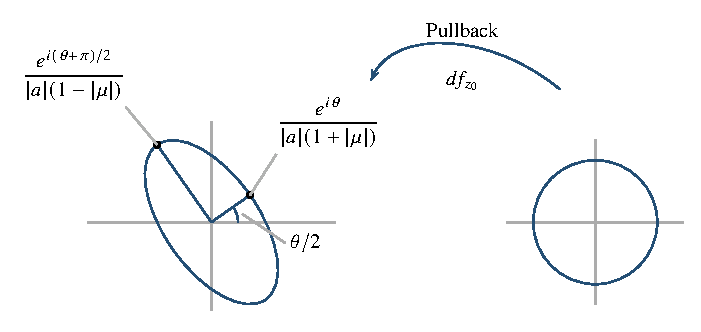
\includegraphics[width=.85\textwidth]{cd10-fig-01.pdf}
\FigureTag{CD10.1}{fig:cd10-01}
\end{figure}
The \emph{dilatation} at \(z_0\) is
\[
K_{z_0}(f):=\frac{\text{major axis}}{\text{minor axis}}
=\frac{1+|\mu_{z_0}|}{1-|\mu_{z_0}|}.
\]
Conformal maps merely dilate and rotate, preserving circles. We propose to study maps that also change their shapes. If
\(\esssup_{z_0\in\mathbb C}K_{z_0}(f)=K<\infty\), then \(K\) measures the failure of \(f\) to be conformal. This could be formalized by introducing Teichm\"uller distance, but we shall not do so here.

% Source page 4
The \(C^1\) assumption was rather unmotivated. There are other ways to ensure that pullback can be done almost everywhere.
\setcounter{definition}{20}\begin{definition}[First analytic definition of quasiconformal maps]
A map \(\varphi:U\to V\) is \(K\)-quasiconformal if it is a homeomorphism, is ACL, and satisfies the ellipse criterion
\[
|\partial_{\bar z}\varphi|\le k|\partial_z\varphi|
\quad\text{almost everywhere},\qquad k=\frac{K-1}{K+1}.
\]
\end{definition}
Why is this the right definition? First, how does one differentiate continuous functions, and what does ACL mean?
\setcounter{definition}{21}\begin{definition}[Absolutely continuous on lines]
A function \(f:U\to\mathbb C\) is \emph{ACL} if, in every rectangle \(R\Subset U\), it is absolutely continuous on almost every line segment in \(R\) parallel to a coordinate axis.
\end{definition}
\begin{remark}
Standard Lebesgue differentiation theory tells us that an ACL function has derivatives almost everywhere. It therefore suffices to require absolute continuity on lines parallel to the \(x\)- and \(y\)-axes.
% Source page 5
Almost-everywhere differentiability along these axes gives the coordinate partial derivatives almost everywhere. Thus \(\partial_zf\) and \(\partial_{\bar z}f\) make sense.
\end{remark}
The definition therefore makes sense. Why it is the right one is the content of what follows.
\setcounter{theorem}{38}\begin{lemma}[Gehring--Lehto]
If \(\varphi\) has partial derivatives almost everywhere and is a homeomorphism, then it is differentiable almost everywhere.
\end{lemma}
\begin{proof}
Consider a bounded measurable region \(\Omega\), of finite measure, and the sequence
\[
\varphi_n(z):=\sup_{0<|h|<1/n}
\left|\frac{\varphi(z+h)-\varphi(z)}h-\varphi_x(z)\right|.
\]
By Egoroff's theorem, \(\varphi_n\) converges uniformly to zero on \(E\), on a measurable set \(E\subset\Omega\) whose complement has arbitrarily small measure. Thus \(\varphi_x,\varphi_y\) are continuous on \(E\), since the difference quotients converge uniformly. Almost every line contains almost every point in \(E\).
For almost every \((x_0,y_0)\in E\), Lebesgue's differentiation theorem gives
\[
\lim_{\substack{m(R)\to0\\(x_0,y_0)\in R}}
\frac1{m(R)}\int_R\mathbf1_E\,dm=1,
\]
where \(R\) is a square of side \(2h\).

% Source page 6
By Fubini's theorem, this becomes
\[
\lim_{\substack{m(R)\to0\\(x_0,y_0)\in R}}
\frac1{m(R)}\int_{y_0-h}^{y_0+h}
\int_{x_0-h}^{x_0+h}\mathbf1_{E_y}(x)\,dx\,dy=1.
\]
Choose \(x_0,y_0\) such that the horizontal and vertical lines through \((x_0,0)\) and \((0,y_0)\) contain almost every point of \(E\) in \(\Omega\). Such points satisfying the limit occur almost everywhere in \(E\). Then
\[
\lim_{h\to0}\frac1{2h}\int_{x_0-h}^{x_0+h}
\mathbf1_{E_{y_0}}(x)\,dx=1.
\]
Thus \(x_0\) is a density point of \(E_{y_0}\), and vice versa. Translate so that \((x_0,y_0)=(0,0)\).
Uniform convergence gives, for \(\varepsilon>0\), a \(\delta>0\) such that
\[
\begin{gathered}
|\varphi_x(z)-\varphi_x(0)|<\varepsilon,\qquad
|\varphi_y(z)-\varphi_y(0)|<\varepsilon,\\
\left|\frac{\varphi(z+h)-\varphi(z)}h-\varphi_x(z)\right|<\varepsilon,\qquad
\left|\frac{\varphi(z+ik)-\varphi(z)}k-\varphi_y(z)\right|<\varepsilon
\end{gathered}
\]
whenever \(|x|,|y|,|h|,|k|<\delta\) and \(z\in E\). The triangle inequality gives
\[
\begin{aligned}
|\varphi(x+iy)-\varphi(0)-x\varphi_x(0)-y\varphi_y(0)|
&\le|\varphi(x+iy)-\varphi(x)-y\varphi_y(x)|\\
&\quad+|\varphi(x)-\varphi(0)-x\varphi_x(0)|\\
&\quad+|y(\varphi_y(x)-\varphi_y(0))|
\le3\varepsilon|z|.
\end{aligned}\tag{*}
\]

% Source page 7
The final inequality holds if
\(|y(\varphi_y(x)-\varphi_y(0))|<\varepsilon|z|\), which holds if \(x\in E\).
We want differentiability at zero, but have shown only
\[
\frac{\left|\varphi(z)-\varphi(0)
-(\varphi_x(0),\varphi_y(0))\binom xy\right|}{|z|}\longrightarrow0
\]
as \(x,y\to0\) with \(x\in E\); similarly with \(y\in E\).
Exploit the fact that zero is a coordinatewise density point of \(E\):
\[
\frac{m(E\cap(-x,x))}{2|x|}\longrightarrow1\quad(x\to0).
\]
There is a \(\delta\) such that, for \(|x|<\delta\),
\[
m(E\cap(-x,x))>\frac{2+\varepsilon}{1+\varepsilon}|x|.
\]
Consequently \((x/(1+\varepsilon),x)\cap E\ne\varnothing\); otherwise
\[
m(E\cap(-x,x))<m((-x,x/(1+\varepsilon)))
=|x|+\frac{|x|}{1+\varepsilon}
=\frac{2+\varepsilon}{1+\varepsilon}|x|.
\]
For \(|z|<\delta/(1+\varepsilon)\), repeat the argument for \((x,(1+\varepsilon)x)\). We may arrange \(x_1,x_2,y_1,y_2\in E\) with
\[
\frac{x}{1+\varepsilon}<x_1<x<x_2<(1+\varepsilon)x,\qquad
\frac{y}{1+\varepsilon}<y_1<y<y_2<(1+\varepsilon)y.
\]
The estimate \((*)\) holds on \(\partial R\), where \(R=(x_1,x_2)\times(y_1,y_2)\).

% Source page 8
The Gehring--Lehto topological lemma for homeomorphisms lets one control this interior error by its boundary values. For \((x,y)\in R\), choose \(z^*=x^*+iy^*\in\partial R\) such that
\[
\begin{aligned}
|\varphi(x+iy)-\varphi(0)-x\varphi_x(0)-y\varphi_y(0)|
&\le|\varphi(z^*)-\varphi(0)-x\varphi_x(0)-y\varphi_y(0)|\\
&\le3\varepsilon|z^*|+|x-x^*|\,|\varphi_x(0)|
+|y-y^*|\,|\varphi_y(0)|\\
&\le3\varepsilon(1+\varepsilon)|z|
+\varepsilon|\varphi_x(0)||z|
+\varepsilon|\varphi_y(0)||z|\\
&=\varepsilon|z|M.
\end{aligned}
\]
This bound is independent of \(z^*\). Therefore \(\varphi\) is differentiable at \((x_0,y_0)\), hence almost everywhere.
\end{proof}

This lemma tells us that quasiconformal maps can pull back circles because they are differentiable almost everywhere. Let \(m=m_1\times m_1\), where \(m_1\) is Lebesgue measure on \(\mathbb R\); naturally \(m\) is Lebesgue measure on \(\mathbb R^2\).
An absolutely continuous function takes a measure-zero subset of an interval to a measure-zero set in its image, directly from the definition.
Locally, let \(\{x\}\times B_x\) have \(m_1\)-measure zero.

% Source page 9
Here \(B_x\) is the projection of the relevant vertical slice of the local region where the measure is zero. Set \(A_x=\{x\}\times B_x\).
Then \(f(\bigcup_{x\in\pi_1(U)}A_x)\) again has measure zero by Fubini, where \(U\) is the local region and \(\pi_1\) is projection onto the first coordinate.
Locally, \(\varphi\) is \(C^1\) almost everywhere by Egoroff and takes measure-zero sets to measure-zero sets. The image of the critical set has measure zero by the area theorem for ACL quasiconformal maps.
Cover \(\mathbb C\) by countably many such local regions. The points where these properties fail still form a measure-zero set, since \(\mathbb C\) is Lindel\"of.

Thus \(K\)-quasiconformal maps pull circles back to ellipses of dilatation at most \(K\). Modulo technical details, this is the right definition: dropping any condition loses something we want. Without a homeomorphism we cannot preserve dynamics. Replacing ACL by existence of partial derivatives almost everywhere does not ensure that critical values form a measure-zero set. Dropping
\(|\partial_{\bar z}\varphi|\le k|\partial_z\varphi|\) loses the meter itself.

% Source page 10
By the Lebesgue decomposition theorem, \(A(E):=m(\varphi(E))\) defines a sigma-finite Borel measure and
\[
A(E)=\int_EJ_\varphi(z)\,dm+\widetilde\mu(E),\qquad
dA=J_\varphi\,dm+d\widetilde\mu,\quad\widetilde\mu\perp m.
\]
Therefore \(\int_EJ_\varphi(z)\,dx\,dy\le A(E)\), where
\(J_\varphi=|\varphi_z|^2-|\varphi_{\bar z}|^2\), and
\[
|\varphi_{\bar z}|^2\le|\varphi_z|^2\le\frac{J_\varphi}{1-k^2}.
\]
Thus \(\varphi_{\bar z},\varphi_z\in L^2_{\mathrm{loc}}\), leading to another definition.
\setcounter{definition}{22}\begin{definition}[Second analytic definition of quasiconformal maps]
A \(K\)-quasiconformal map \(\varphi:U\to V\) is an orientation-preserving homeomorphism in \(W^{1,2}_{\mathrm{loc}}(U)\) satisfying
\(|\varphi_{\bar z}|\le k|\varphi_z|\), the ellipse criterion.
\end{definition}
The analytic definitions are useful only to an extent. A promising alternative, with its own limitations, is the geometric definition.
\setcounter{definition}{23}\begin{definition}[Geometric definition of quasiconformal maps]
An orientation-preserving homeomorphism \(\varphi:U\to V\) is \(K\)-quasiconformal if
\[
\frac1K\operatorname{mod}Q
\le\operatorname{mod}\varphi(Q)
\le K\operatorname{mod}Q
\]
for every topological quadrilateral \(Q\Subset U\).
\end{definition}
After conformally identifying a quadrilateral with a rectangle, its modulus is the rectangle's ratio of length to breadth.

% Source page 11
The analytic definition makes it obvious that quasiconformality is local, whereas this is extremely nontrivial to derive geometrically. Conversely, the geometric definition makes it obvious that \(\varphi^{-1}\) is \(K\)-quasiconformal, which is not immediate analytically.
The three definitions can be proved equivalent; we skip the proof to preserve the flow.

To ensure that our meter measures conformality and is not an artificial monster, we must recover conformality by reversing what we adjusted. The following powerful lemma ensures this.
\setcounter{theorem}{39}\begin{lemma}[Weyl's lemma]
A \(1\)-quasiconformal map is conformal.
\end{lemma}
\begin{proof}[Proof sketch]
By the equivalence of definitions, it suffices to prove that a map \(\varphi\) with \(\partial\varphi/\partial\bar z=0\) in the sense of distributions is conformal. Fix a compact disc on which a cutoff \(\eta\) is identically one, and construct
\(f_n=\varphi_n*(\eta f)\), where \(\varphi_n\) is a scaled mollifier. Then \(f_n\) is smooth and \(f_n\to f\) in \(L^1\) on compact sets. On every smaller disc and for all sufficiently large \(n\),
\[
(f_n)_{\bar z}=\varphi_n*f_{\bar z}=0.
\]
Thus the smooth functions \(f_n\) are holomorphic there. Their distributional limit is \(f\), so Weyl's lemma gives a holomorphic representative of \(f\).
\end{proof}

% Source page 12
This ensures that the meter for conformality is dilatation! Next we shall see why we need to loosen the conformality condition.
% BLOG-CONTENT-END
\end{document}
